\section{Alur Konversi Spesifikasi}

Dalam bagian ini, penulis membahas bagaimana alur konversi dari spesifikasi hingga menjadi suatu kode sistem yang siap digunakan.
Alur konversi ini akan dijadikan landasan dalam proses implementasi kakas.
Berikut adalah gambaran alur penggunaan kakas secara umum melalui diagram konteks dari kakas ini.

\begin{figure}[H]
    \centering
    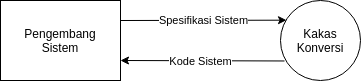
\includegraphics[width=0.4\textwidth]{resources/images/chapter-3/03-diagram-konteks.drawio.png}
    \caption{Diagram Konteks Kakas}
\end{figure}

Untuk lebih rincinya, penulis membuat diagram aliran data (\textit{Data Flow Diagram}) untuk tahap konversi dari spesifikasi.
Hal yang perlu menjadi perhatian utama adalah tahapan konversi kakas dalam melakukan pemetaan data masukan dan \textit{pipeline} pemrosesan data.
Berikut ini adalah alur penggunaan tiap komponen dalam spesifikasi ketika dilakukan konversi menggunakan kakas. 

\begin{figure}[H]
    \centering
    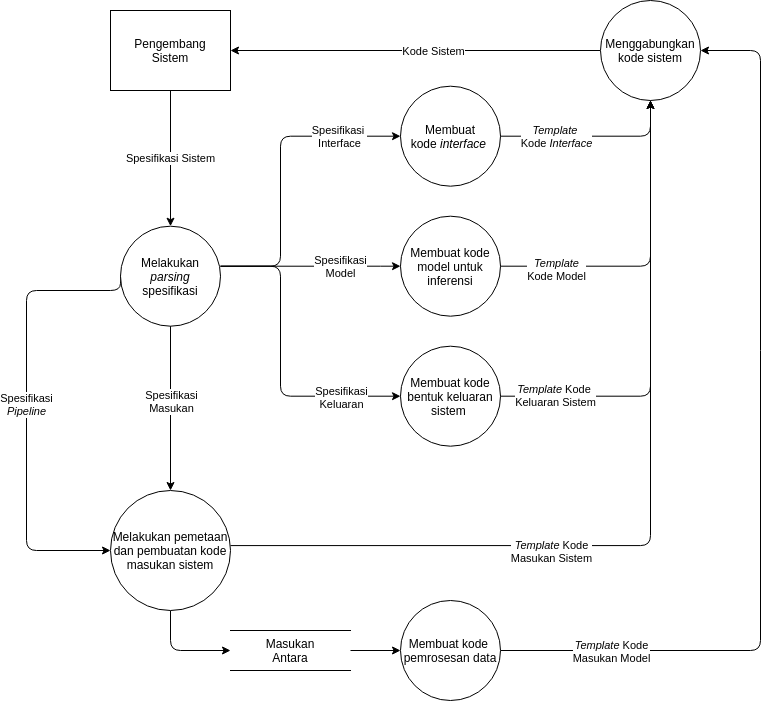
\includegraphics[width=0.9\textwidth]{resources/images/chapter-3/03-diagram-pembacaan-spesifikasi.drawio.png}
    \caption{Diagram Konteks Kakas}
\end{figure}